
\chapter{Vision}
\section{Optical Flow}
\subsection{useful links}
\url{https://stackoverflow.com/questions/47465570/opencv-feature-matching-vs-optical-flow}.
\url{http://www.cad.zju.edu.cn/home/gfzhang/course/computational-photography/}.
\url{https://ags.cs.uni-kl.de/fileadmin/inf_ags/opt-ss12/lec05_opt.pdf}.
\url{http://people.csail.mit.edu/celiu/SIFTflow/ SIFT Flow}.
\url{https://www.reddit.com/r/computervision/comments/9n4o6p/optical_flow_vs_feature_matching_in_sparse_voslam/}.

\textcolor{blue}{So, basically speaking, optical flow is ok for small motion while feature matching can work with very large motion. From the comparison of running optical flow on the dataset captured by matrixvision and gopro, on mvision, although coarse-to-fine optical flow can track a certain number of features, but if I do a loop check (frame1 to frame2 and then backward from frame2 to frame1, and compare the result, theoretically, they should be the same or very small), I found very big error. However, on Gopro dataset, the optical flow works pretty well. The only difference is the FPS, gopro has 30 while mvision only has 10. So a small motion to gopro may mean a big motion to mvision. Another lesson learned from this experiment is the trade off between the tracking accuracy(winSize: small accurate) to the robustness (large window size tolerate large motion).}

\subsection{Tracking}
For optical flow, I use the LK tracker for constructing features correspondences. The lesson learned here is that the tracking results may contains severe wrong matches. So a loop fashion is favoured: 
\begin{itemize}
	\item do forward LK tracking from last frame to current frame;
	\item do backward LK tracking from current frame to last frame;
	\item check if the forward-backward feature point corresponds to the original feature point in the last frame by checking the relative distance; 
\end{itemize}
This can eliminate large number of wrong tracks.

\subsection{RANSAC}

\subsection{Homography}

\subsection{Fundamental Matrix}
The importance of applying normalization for fundamental matrix estimation was given in~\cite{hartley1995defence}.

\subsection{Essential matrix}
Two methods are implemented for essential matrix estimation: the $8$-point algorithm and the $5$ point algorithm~\cite{nister2003efficient}~\cite{li2006five}~\cite{triggs2000routines}~\cite{nister2004efficient}. $8$ point algorithm is chosen since it is the most straight-forward method which gives only one solution, while $5$ point algorithm is the minimal solution for essential matrix estimation. It is easy to derive from $5$ point algorithm to other $6$ or $7$ point algorithms, although the $6$ or $7$ point algorithms were proposed earlier than $5$ point algorithms.

\subsubsection{$5$ point algorithm}
TODO a brief summary of $5$ point algorithm.

The most widely known $5$ point algorithms or implementations are listed here:
\begin{enumerate}
\item Nist\'er version in CVPR~\cite{nister2003efficient} and PAMI~\cite{nister2004efficient}. The PAMI version is favoured here since it is relatively simpler.
\item Gr\"obner basis version in~\cite{stewenius2006recent}. 
\item Polynomial Eigenvalue solution in~\cite{kukelovapolynomial}.
\end{enumerate}
Implementations:
\begin{itemize}
\item \url{https://github.com/prateekt/allyourposesrours}: a \textsc{Matlab} symbolic based implementation of Nist\'er five point algorithm.
\item archived at \url{https://web.archive.org/web/20170401223934/http://www.vis.uky.edu:80/~stewe/FIVEPOINT/}: a \textsc{Matlab} based Grobner Basis Method and a Nist\'er five point implementation.
\item \url{https://raw.githubusercontent.com/jianxiongxiao/SFMedu/master/peig5pt.m}: Polynomial Eigenvalue solution.
\item: two self developed implementations.
\end{itemize}
A performance and runtime evaluation can be seen from
\begin{figure}
\centering
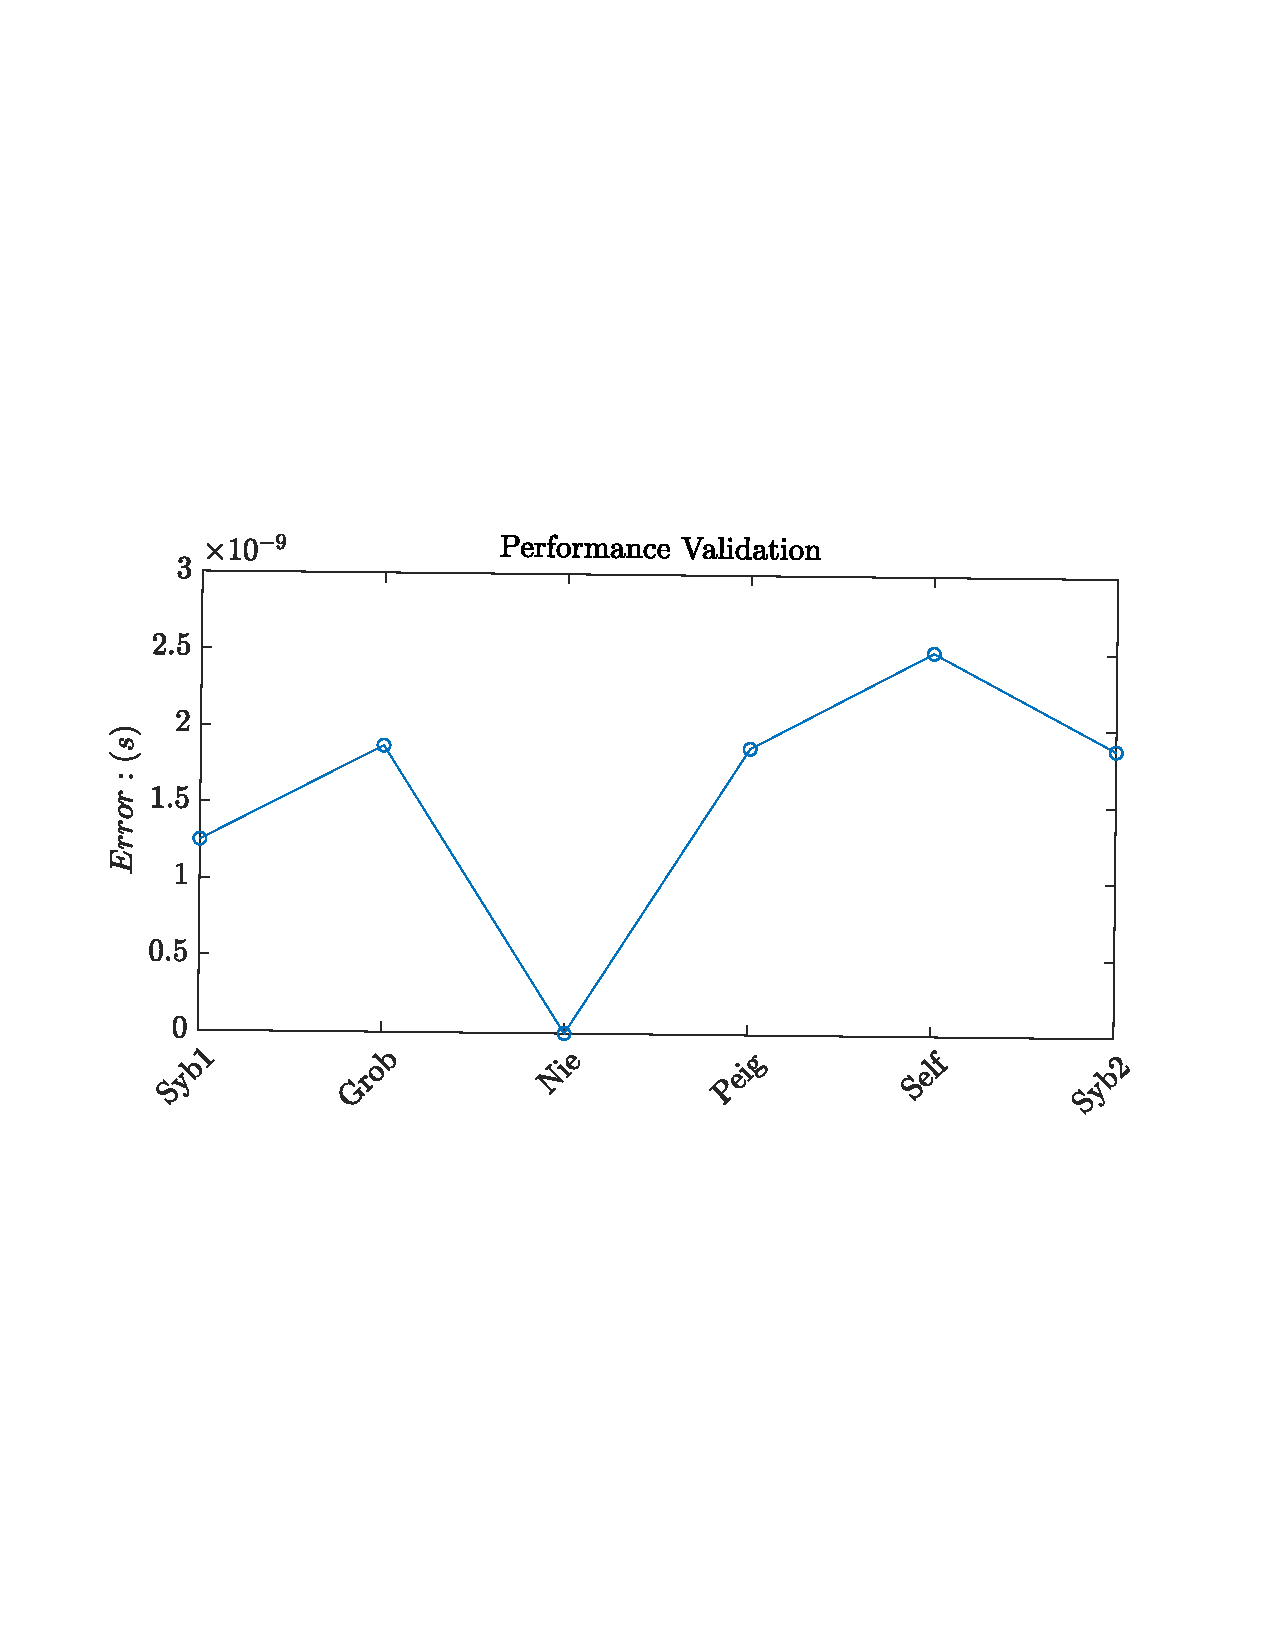
\includegraphics[width=0.45\textwidth]{hand_eye_files/vision/figures/five_point_perf}
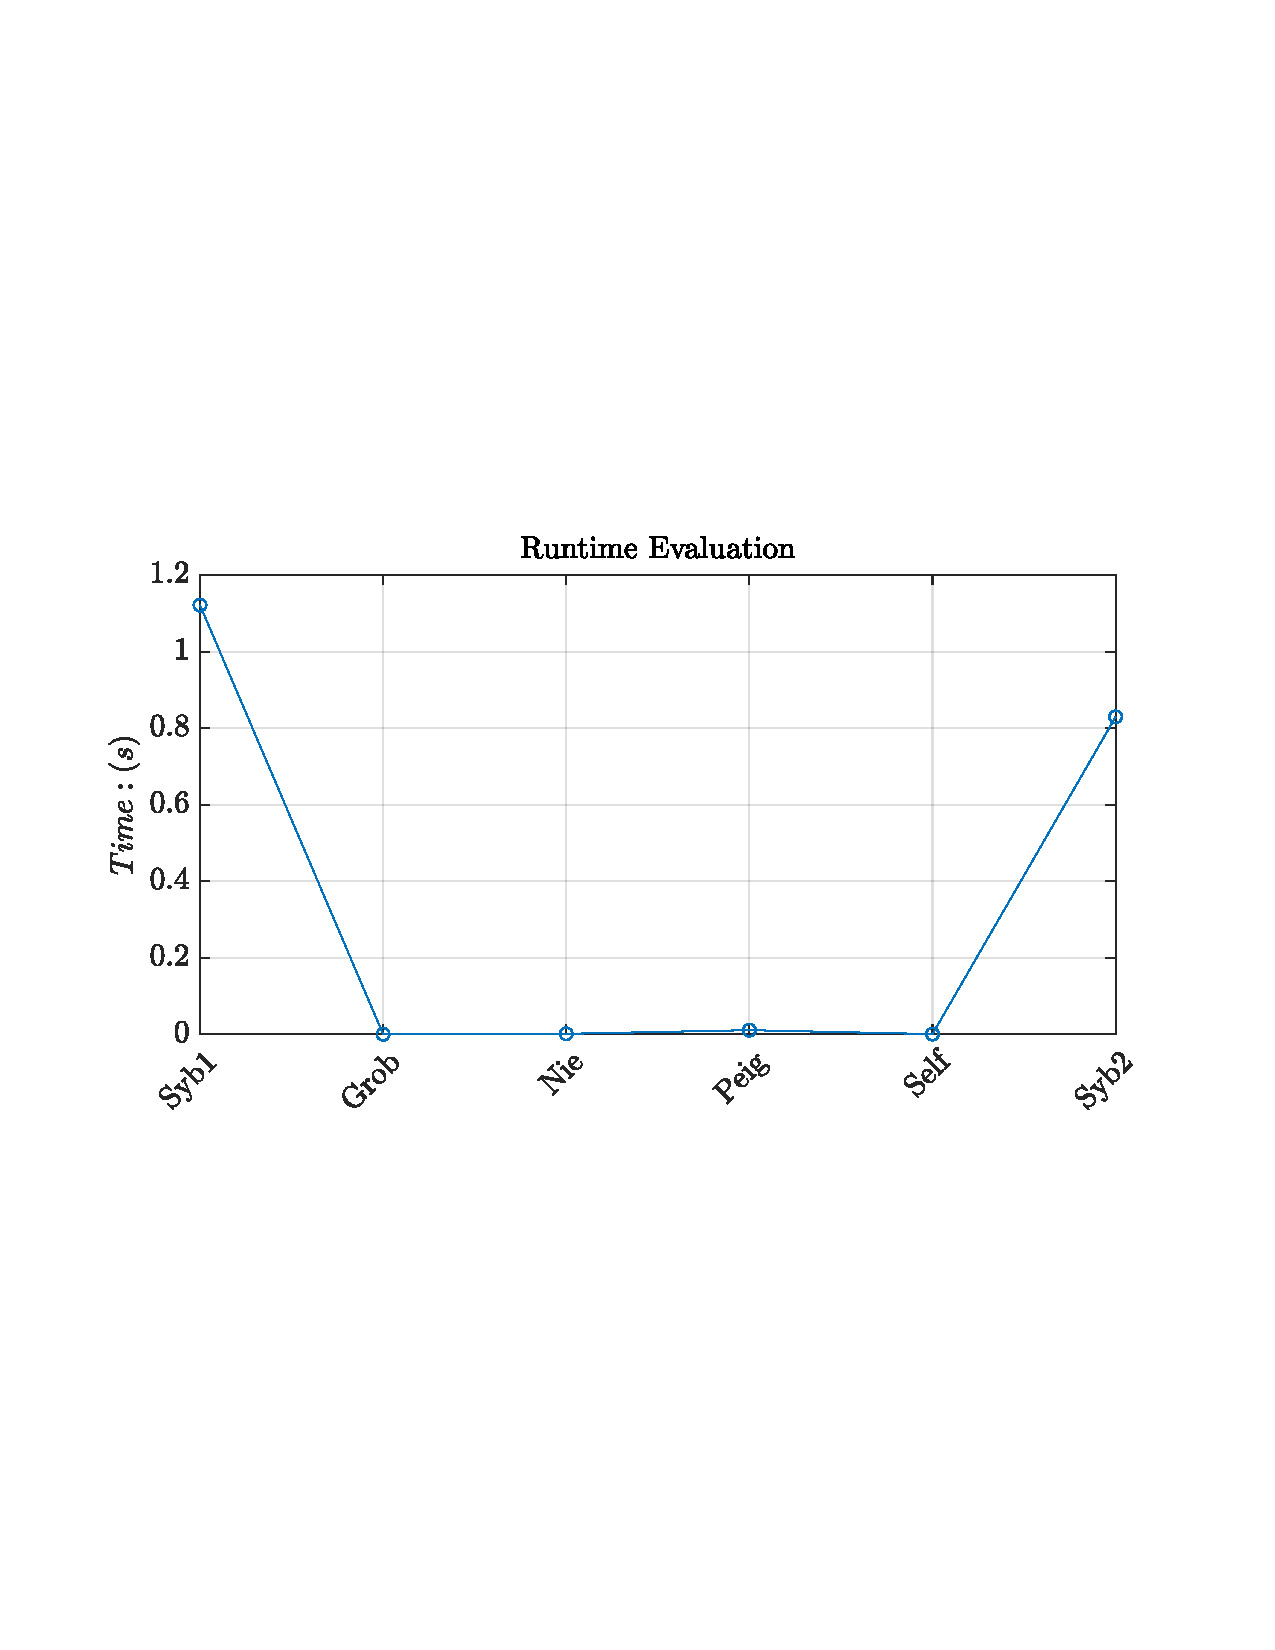
\includegraphics[width=0.45\textwidth]{hand_eye_files/vision/figures/five_point_time}
\label{fig:ess_com}
\end{figure}
\begin{table}[h!]
\centering
\caption{Details of runtime}
\begin{tabular}{c||c}
\hline
\textbf{Name} & \textbf{Time}: (s) \\
 Syb1 & $1.1213$ \\
 Grob & $0.0002$ \\
 Nie & $0.0015$ \\
 Peig & $0.0110$ \\
 Self & $0.0008$ \\
 Syb2 & $1.8294$ \\ 
 \hline
\end{tabular}
\label{tb:ess_com}
\end{table}
From this figure~\ref{fig:ess_com} and Table~\ref{tb:ess_com}, it can be seen Grob, Nie, Self are the three fastest methods. So they are chosen as the five point algorithm for future usage\footnote{$100$ Experiments are carried for evaluation.}.

\subsubsection{Composition}
\subsubsection{Computation}
\subsubsection{Tracking with special linear group}

\subsection{KD-Tree}
Since many computer vision tasks needs to find the correspondance and the low efficiency of brute-force search, KD tree is often used for boosting the searching procedure. Basically speaking, KD tree is a data structure which manages data by dividing the space into several sub-spaces. There are several stable and popular open source implementation of KD tree available on github:
\begin{itemize}
\item \textbf{nanoflann}\footnote{\url{https://github.com/jlblancoc/nanoflann}}
\item \textbf{FLANN}\footnote{\url{http://www.cs.ubc.ca/research/flann/}}: ANN for C, Matlab.
\item \textbf{kdtree}\footnote{\url{https://github.com/jtsiomb/kdtree}}: pure C implementation, I have once used this for path planning.
\end{itemize}
I have chosen \textbf{nanoflann} for KD tree implementation for program in \textsc{C/C++} and \textbf{FLANN} for ANN tree for program in \textsc{Matlab}.

Usage of \textbf{nanoflann}:
\begin{itemize}
\item create a kd-tree index: must specify distance template, data source type and dimension.
\item add points in chunks or build index;
\item 2 types of search: find nearest neighbours and find in radius;
\end{itemize}
SO3 is supported with quaternion and SO2 is supported with $\theta$.

\subsection{Feature \& Descriptor}
A fairly simple compare of commonly used features are given by\footnote{\url{https://marcosnietoblog.wordpress.com/}}.
I plan to try with \textbf{FAST}+\textbf{BRIEF} and \textbf{ORB}.
It could be very beneficial to read the source code of some feature detections and feature descriptions.

\subsection{Matching}
Normally, the matched correspondances would contain large number of wrong matches. The conventional methods which can mitigate this problem include:
\begin{enumerate}
	\item left-right check or even round check: match left to right then right to left, or previous to current and current to previous, and check if the corresponding point will round back to the original point. If not, consider a mismatch. This is robust, but time-consuming.
	\item uniqueness: find 2 best matches, only accept the match if the best score if significantly smaller than the second best score.
	\item na\"{\i}ve method including compute the mean and standard deviation of the distance and then filter out matches whose distance is beyond a threshold. This can also be done to compute mean and standard deviation of the displacement between two frames.
	\item use epipolar constraint or use homography constraint: the idea is to compute the fundamental or homography matrix and then corresponding distances. Filter out matches whose distance is over a threshold. This should be the most time consuming approach.
\end{enumerate}
\textcolor{blue}{It is better to see if some one can test this}.